\subsection{Umweltmodellierung}
\begin{figure}[ht]\centering 
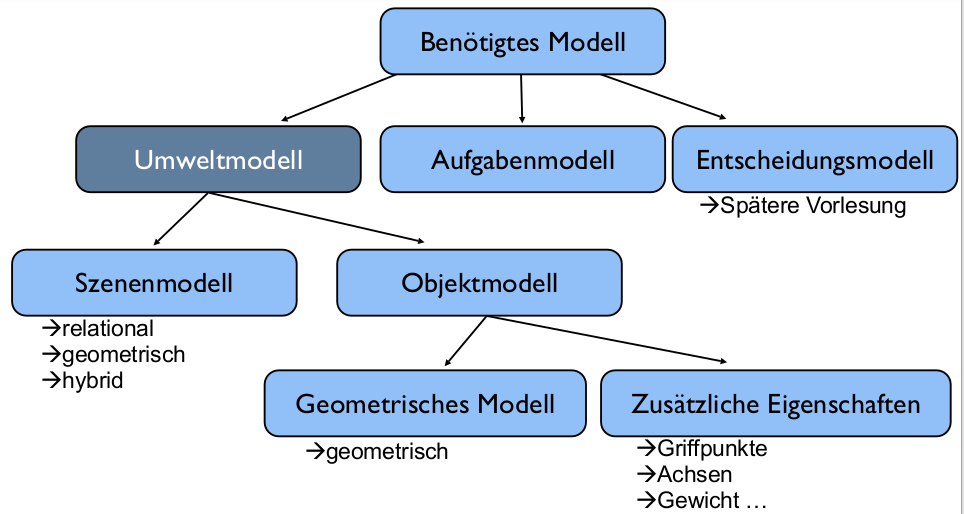
\includegraphics[width=0.6\linewidth]{figures/ch02_umweltmodell.png}
\caption{Umweltmodell}
\label{fig:ch02_um}
\end{figure}

%Keine Umlaute in labels!!!
\subsubsection{Objektmodell}
Die geometrische Beschreibung von Objekten beinhaltet:
\begin{itemize}
\setlength\itemsep{0em}
\item graphische Darstellung
\item Kollisionsberechnungen, Kontaktberechnung in Griffplanung, ...
\item physikalisch-dynamische Simulation der Effekte von Handlungen auf die Umwelt
\item geometriebezogene Bewegungsplanung
\end{itemize}
Es gibt drei Ansätze zur geometrischen Modellierung: Kantenmodelle, Flächenmodelle und Volumenmodelle.\\
\paragraph*{Kanten}
Nur die Kanten werden gespeichert, d.h. Punkte und Verbindungen (Gerade, Polygonzug, Bezierkurve, ... ).
\begin{table}[hbt]
\centering
\begin{tabular}{|p{6.5cm}|p{6.5cm}|}
\hline
Vorteile & Nachteile\\
\hline
\vspace{-5mm}
\begin{itemize}
\setlength\itemsep{0em}
\item[+] einfache Daten
\item[+] wenige Daten
\end{itemize}
 &
 \vspace{-5mm}
\begin{itemize}
\setlength\itemsep{0em}
\item[-] Mehrdeutigkeiten
\item[-] hoher Eingabeaufwand
\item[-] keine Kollisionsberechnung
\item[-] kein Schnitt
\end{itemize}\\
\hline
\end{tabular}
\caption{Zusammenfassung: Kantenmodelle}
\label{tab:Kantenmod}
\end{table}\\ 
\paragraph*{Flächen}
Flächen können exakt modelliert werden, wenn sie \textcolor{red}{analytisch gegeben} sind (eine 3D Kugel beispielsweise durch $r = ||x-p||$, wobei $r$ der Radius und $p$ der Mittelpunkt ist).
\begin{table}[hbt]
\centering
\begin{tabular}{|p{6.5cm}|p{6.5cm}|}
\hline
Vorteile & Nachteile\\
\hline
\vspace{-5mm}
\begin{itemize}
\setlength\itemsep{0em}
\item[+] Geschlossene Darstellung (wenig Speicherbedarf)
\item[+] Analytische Darstellung erlaubt einfache Rechenverfahren (z.B.
Schnitt von Ebenen / Kugeln $\rightarrow$ schnelle Kollisionsberechnung)
\end{itemize}
 &
 \vspace{-5mm}
\begin{itemize}
\setlength\itemsep{0em}
\item[-] Wenige Flächen sind analytisch darstellbar
\end{itemize}\\
\hline
\end{tabular}
\caption{Flächen: analytisch}
\label{tab:Flaechen-analyt}
\end{table}\\ 
Ansonsten werden sie \textcolor{red}{approximativ} durch Bildung einer großen Fläche aus einem Netz (\glqq Mesh\grqq ) von einfachen Einzelflächen, z.B. Dreiecke, Vierecke modelliert.\\
\begin{table}[hbt]
\centering
\begin{tabular}{|p{6.5cm}|p{6.5cm}|}
\hline
Vorteile & Nachteile\\
\hline
\vspace{-5mm}
\begin{itemize}
\setlength\itemsep{0em}
\item[+] Definition sehr einfach
\item[+] einfache Algorithmen
\end{itemize}
 &
 \vspace{-5mm}
\begin{itemize}
\setlength\itemsep{0em}
\item[-] hoher Speicherbedarf
\item[-] hoher Rechenaufwand
\end{itemize}\\
\hline
\end{tabular}
\caption{Flächen: approximativ}
\label{tab:Flaechen_approx}
\end{table}\\ 
Hierbei werden Freiformflächen im einfachsten Fall durch \textit{Dreiecksflächen} approximiert:
Gegeben seien 3 Punkte im Raum $P_1 , P_2 , P_3$. Damit hat die Fläche folgende Gleichung:
$F(u,v)=u\cdot P_1 +v\cdot P_2 +(1-u-v)\cdot P_3$ mit $0 \leq u,v, u+v \leq 1$.\\
Oder sie werden durch \textit{Bilineare Viereckselemente / Pflaster} approximiert:
Gegeben sind 4 Punkte im Raum $P_1 , P_2 , P_3, P_4$
Damit wird die Fläche definiert durch $F(u,v)=(1-u)(1-v) \cdot P_1 + (1-u)v \cdot P_2 + u(1-v) \cdot P_3 + uv \cdot P_4$ mit $0 \leq u \leq 1, 0 \leq v \leq 1$. 
\begin{table}[hbt]
\centering
\begin{tabular}{|p{6.5cm}|p{6.5cm}|}
\hline
Vorteile & Nachteile\\
\hline
\vspace{-5mm}
\begin{itemize}
\setlength\itemsep{0em}
\item[+] Flächenelemente können gekrümmt sein
$\rightarrow$ weniger Gitterpunkte bei gleich guter Approximation
\end{itemize}
 &
 \vspace{-5mm}
\begin{itemize}
\setlength\itemsep{0em}
\item[-] Rechnen mit gekrümmten Flächen ist aufwendig
\end{itemize}\\
\hline
\end{tabular}
\caption{Approximation durch Vierecke}
\label{tab:Viereck_approx}
\end{table}\\
Zudem können Flächen durch Bezierflächen, einer Erweiterung der Bezierkurven beschrieben werden: Gegeben ist ein Gitter von Führungspunkten $P_{ij}, 0 \leq i \leq N$ und $0 \leq j \leq M$. Damit ist die Fläche beschrieben durch $F(u,v) = \sum_{i=0}^N \sum_{j=0}^M P_{ij} \cdot B_{i,N}(u) \cdot B_{j,M}(v)$ mit $B_{i,N}(u) = (1-u)B_{i,N-1}(u)+uB_{i-1,N-1}(u)$ und
$B_{j,M}(v) = (1-v)B_{j,M-1}(v)+vB_{j-1,M-1}(v)$.\\ Die $B_{i,N}$ bzw. $B_{j,M}$ heißen auch Bernsteinpolynome.
\begin{table}[hbt]
\centering
\begin{tabular}{|p{6.5cm}|p{6.5cm}|}
\hline
Vorteile & Nachteile\\
\hline
\vspace{-5mm}
\begin{itemize}
\setlength\itemsep{0em}
\item[+] effiziente Verfahren 
\item[+] entspricht dem Vorgehen während der Modellierung
\item[+] schnelle Kollisions- und Abstandsberechnung
\end{itemize}
 &
 \vspace{-5mm}
\begin{itemize}
\setlength\itemsep{0em}
\item[-] hoher Eingabeaufwand
\item[-] Darstellung aufwendig
\item[-] Problem bei Schnittoperationen
\item[-] Inkonsistenzen möglich
\end{itemize}\\
\hline
\end{tabular}
\caption{Zusammenfassung: Flächenmodelle}
\label{tab:Flaechenmod}
\end{table}\\ 

\paragraph*{Volumen} Vier verschiedene Arten von Volumenmodellen:\\
\textit{Parametrische Modelle}: Grundkörper und topologische Operationen auf diesen (Schnitt, Vereinigung, ... ) werden abgespeichert. DIe Objekte sind bereits vorhanden und können durch Angabe von Parametern angepaßt werden (Varianten). Konsistenzprüfungen sind notwendig ! (Bsp auf F20)
\begin{table}[hbt]
\centering
\begin{tabular}{|p{6.5cm}|p{6.5cm}|}
\hline
Vorteile & Nachteile\\
\hline
\vspace{-5mm}
\begin{itemize}
\setlength\itemsep{0em}
\item[+] eindeutige Objektbeschreibung 
\item[+] geringer Eingabeaufwand 
\item[+] Ergebnis von Operationen sind korrekte Objekte
\end{itemize}
 &
 \vspace{-5mm}
\begin{itemize}
\setlength\itemsep{0em}
\item[-] hoher Implementierungsaufwand
\item[-] Einbindung von Freiformflächen schwierig
\end{itemize}\\
\hline
\end{tabular}
\caption{Volumenmodelle: parametrisch}
\label{tab:Volmod}
\end{table}\\ 
\textit{Zellenzerlegung}: Objekte werden aus disjunkten Elementarzellen aufgebaut. Verwendung finden einfache geometrische Objekte z,B. Tetraeder, Quader, ...
Benutzt in der Strukturanalyse mit Finite-Elemente-Methoden (FEM).
\textit{Boundary Repräsentation}: Hierarchische Darstellung eines Objektes durch begrenzende
Elemente, i.d.R. Kanten oder Flächen. (Bsp. auf F23)
Die Vorteile von B-Rep sind, dass man aus der topologischen Struktur Information über z.B.:
\begin{itemize}
\item Welche Flächen gehören zum Objekt?
\item Welche Kanten gehören zur Fläche?
\item Zu welchem Objekt gehört eine Fläche?
\item Zu welchem Objekt gehört eine Kante?
\item Welche Flächen stoßen aneinander?
\end{itemize}
erhält.\\
\textit{Constructive Solid Geometry (CSG)}:
Es gibt eine Menge von einfachen Grundkörpern, die parametriert
werden können (Bsp. F26, 27) und auf denen verschiedene Operationen definiert sind, z.B.
\begin{table}[hbt]
\centering
\begin{tabular}{|p{6.5cm}|p{6.5cm}|}
\hline
Objekt $A$ & Objekt $B$\\
\hline
Vereinigung $A \cup B$ (Summe) & Bild\\
\hline
Schnitt $A \cap B$ & Bild \\
\hline
Differenz $A / B$ & Bild\\
\hline
Sweep:
Ein Grundelement (u.U. eine Fläche) wird entlang einer Raumkurve
verschoben. Der durchdrungene Raum stellt das neue Objekt dar. & \\
\hline
\end{tabular}
\caption{CSG: Operatoren}
\label{tab:csg_ops}
\end{table}\\ 
\textit{Zellenbelegung}:
Der Raum wird in mehrere Zellen unterteilt (i.d.R. 8 Zellen: \glqq Octree\grqq{}).
Wenn eine Zelle komplett vom Objekt belegt ist, als \glqq belegt\grqq{} markieren.
Wenn die Zelle nur teilweise belegt ist, dann wird auf diese Zelle das
Verfahren rekursiv angewendet. Ansonsten ist die Zelle leer.
Die Rekursion terminiert bei einer vorbestimmten minimalen Zellgröße.
Teilbelegte kleinste Zellen werden als belegt markiert. (Bsp. F28, 29)
\subsection{Aufgabenmodellierung}
\begin{figure}[ht]\centering 
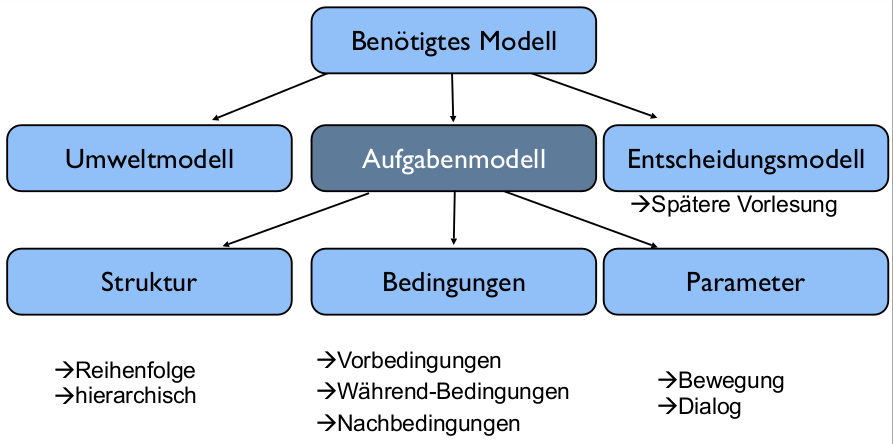
\includegraphics[width=0.6\linewidth]{figures/ch02_aufgabenmodell.png}
\caption{Aufgabenmodell}
\label{fig:ch02_am}
\end{figure}
%kognitive Lücke?
\begin{figure}[ht]\centering 
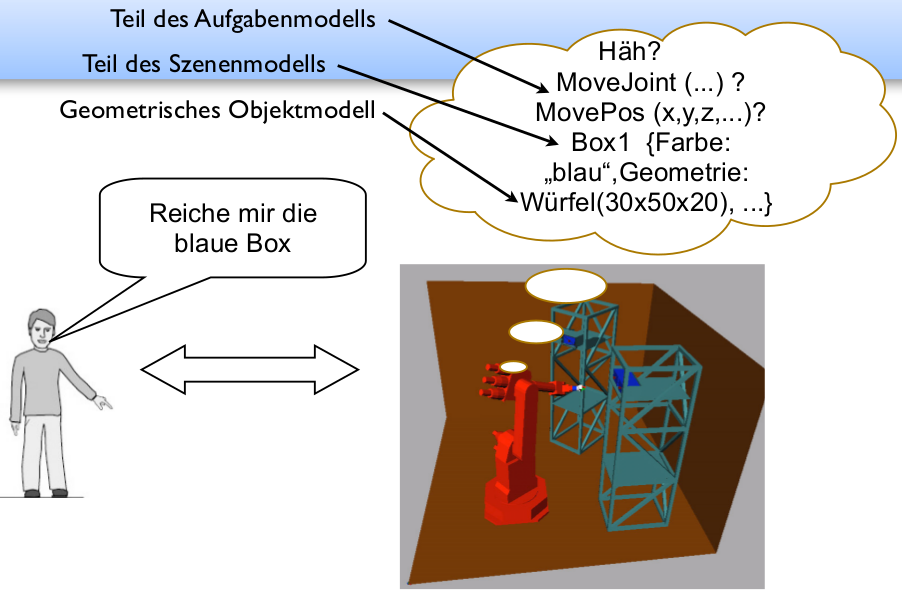
\includegraphics[width=0.6\linewidth]{figures/ch02_beispiel.png}
\caption{Beispiel}
\label{fig:ch02_bsp}
\end{figure}
\begin{figure}[ht]\centering 
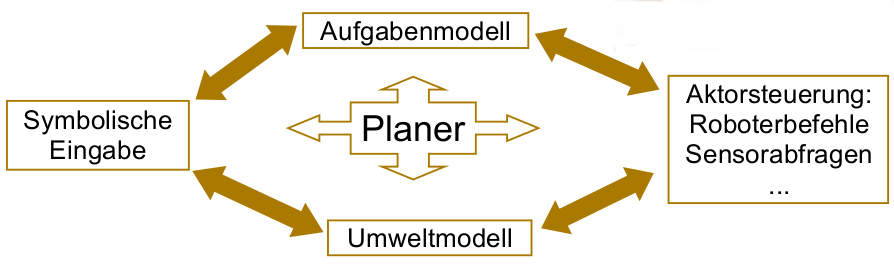
\includegraphics[width=0.6\linewidth]{figures/ch02_planer.png}
\caption{Einordnung des Aufgabenmodells}
\label{fig:ch02_ord}
\end{figure}
\textit{Symbolische Abstraktion}: Benutzer beschreibt die Aufgabe mit seinen Worten (z.B. \glqq Bring mir Tee!\grqq) $\rightarrow$ Abbildung: Erzeugung der Roboterbefehle über mehrere Stufen:\\
$\rightarrow$ \glqq Fahre in die ‚Küche‘, greife ein Glas, fahre zurück und reiche mir den Becher.\grqq \\
$\rightarrow$ \glqq DriveTo(...), SearchObject(...), MoveArm(...), Grasp(Becher), MoveArm(...), DriveTo(...), MoveArm(...) ...!\grqq \\

\textit{Modellierung der Reihenfolge von Operatoren/Symbolische Handlungsatome}:
\begin{itemize}
\item In den gegebenen Beispielen wurden bereits implizit Handlungsatome angenommen
\item Die kleinsten auszuführenden Handlungseinheiten werden als
Elementaroperationen oder atomare Handlungen bezeichnet.
\item Komplexe Handlungen werden aus Elementaroperationen zusammengesetzt. Diese
können dazu üblicherweise parametriert werden.
\item Jeder Roboter besitzt eine endliche Menge an Elementaroperationen.
\end{itemize}
Makro-Operatoren
Abstraktionsebenen im Aufgabenmodell
Validierung der Modelle: Simulation oder Graphische Animation

-------
Aufgabenmodell basiert auf elementaren Operationen
Oft dreischichtiger Ansatz: Aktion, Task, Mission
Verknüpfung der elementaren Operationen zu komplexen Aufgaben
Verknüpfung:

Sequentiell
Vorranggraph
Hierarchisch
(Kontrollstrukturen)
Problem: Validierung der Programme
Simulation
Animation und Validierung durch den Menschen
%